\chapter{小缓冲区组技术}
\label{chap:sba}

存储介质性能的发展要求比传统系统更轻薄的存储软件栈,以更好地发挥硬件提供的更高的吞吐能力和更低的访问延迟。我们提出将一个可扩展的事务性内存系统直接架构在大容量非易失性存储设备上以达到上述要求。我们的解决方案绕开了复杂的代价高昂的数据库系统,应用程序可直接使用事务;并且解决了传统持久性事务性内存系统在可扩展性和容量方面的局限。系统假设市面上现成的存储设备,并基于我们对最新的接口和存储设备的特性的观察。我们通过两项技术改进了持久性事务性内存系统一致性机制的可扩展性和效率:
(1)采用我们事务性内存系统的\emph{快照隔离}机制使得持久化的开销对只读负载隐藏;
(2)设计了共享的\emph{小缓冲区组技术}供预写式日志使用。该缓冲区设计在满足一致性要求的同时,面向事务性内存系统设计,可以同时实现高吞吐率和低延迟的特性。

\section{可扩展的持久性事务性内存系统}

存储系统对应用的性能有显著影响。两个硬件发展的新趋势增强了这方面影响。首先,非易失性存储(例如闪存\cite{Chen:2009:UIC:1555349.1555371, 4804997}、ReRAM\cite{6327378, 7168603}、PCM\cite{Loke22062012,6176872,Raoux:2008:PRA,10.1109/MM.2010.24}、STT-RAM\cite{4443191,6557176}等)极大扩展了传统存储系统的带宽,降低了访问延迟,相应地也要求高效的系统软件来充分利用这些优势。其次,多核和多处理器架构需要存储软件层的可扩展性来匹配上层应用的可扩展性\cite{Zheng:2014:FDF:2685048.2685085,Kimura:2015:FOE:2723372.2746480}。

最初事务性内存系统的提出是用于并发控制,为了简化基于锁的程序的设计和编码。由于持久化的开销较高,传统事务性内存中的事务并不提供持久性的保证,而仅仅保证ACID中的另外三项:原子性、一致性和隔离性。而应用程序需要使用其他事务性系统,例如数据库,来完成数据持久化的需求。这种使用模式和厚重的数据库系统带来可观的系统开销,而且随着高速存储硬件的发展日益成为系统性能的瓶颈。相较于轻量级的事务性内存系统,数据库系统可能带来几十倍的性能降低\cite{Volos:2011:MLP:1950365.1950379,
Coburn:2011:NMP:1950365.1950380}。

因此,完整支持ACID的事务性内存系统,作为应用程序访问持久性数据的新接口,得到广泛的关注和研究\cite{Volos:2011:MLP:1950365.1950379,
Coburn:2011:NMP:1950365.1950380, Zhao:2013:KCP:2540708.2540744, 6828760}。然而,现有的此类系统多依赖于新型的可字节访问的非易失性内存(例如ReRAM、PCM、STT-RAM等)。新型非易失性内存尚未普遍商业应用,在价格、容量等方面有诸多限制(例如Intel-Micro最新推出的3D XPoint非易失性内存单片容量128GB)。而闪存、固态硬盘等按块访问的非易失性存储设备已经非常成熟,价格低廉,在基于PCIe的NVMHCI 或NVMe~\cite{nvme}的最新接口技术下容量和扩展性都更加理想。

本章提出一种基于当前商业应用的非易失性存储的持久性事务性内存,具备并发能力、吞吐能力和容量的高可扩展性。我们采用预写式日志的方式来实现数据的持久性以及保证持久性数据的一致性,并改进了缓冲区的设计,解决了持久性和一致性机制的性能瓶颈。

我们面临两方面的挑战。第一,商业可用的非易失性存储,如基于闪存的固态硬盘,虽然容量可扩展性高,但其写入延迟仍然是远不可忽略的问题,比新型的可字节访问的非易失性内存介质要高两个以上的数量级。在一个事务性内存系统中直接应用当前商业可用的非易失性存储并不可行,需要我们将持久化的开销尽量隐藏起来。系统吞吐性能之所以对持久化开销很敏感,原因是写事务需要锁住所有相关的写锁直到其预写式日志项完成持久化。这很容易成为系统性能瓶颈\cite{Chen:2009:FEF:1559845.1559855,
Johnson:2010:ASA:1920841.1920928, Johnson:2012:SWL:2205457.2205463,
Zheng:2014:FDF:2685048.2685085},并且这种由于日志导致的锁行为\cite{Johnson:2010:ASA:1920841.1920928}被广泛定位为线程竞争等待的一个主要原因。第二,传统集中式大体积的日志缓冲区在高并发的使用环境下会导致低效的缓冲区竞争\cite{Johnson:2010:ASA:1920841.1920928,
Huang:2014:NLT:2735496.2735502}。该设计思想主要来自于机械硬盘顺序写性能的突出优势,并不于非易失性存储的特性相符合。采用线程局部的缓冲区\cite{Johnson:2012:SWL:2205457.2205463,
Zheng:2014:FDF:2685048.2685085, Wang:2014:SLT:2732951.2732960}需要单个线程执行多个事务来填充其独占的缓冲区以进行组提交,与事务性内存简单的线程模型相违背。而且,它依然需要不同线程间进行事务级的协调\cite{Johnson:2012:SWL:2205457.2205463,Wang:2014:SLT:2732951.2732960}。

为了应对第一个挑战,我们在事务性内存系统中采用快照隔离技术。特别地,我们维护一致的数据历史版本,只读的事务在一个历史快照上执行,不会与其他事务冲突,可以直接提交。相对于传统将动态写入数据定期归档进数据仓库再进行分析的模式,当前实时性分析与动态写入数据混合的模式\cite{ren2011querying,
Cheng:2012:KTP:2168836.2168846,4302625,Corbett:2012:SGG:2387880.2387905}更能体现出我们系统避免持久化写事务拖累读事务的优势。我们的系统可以显著提高此类负载下的综合吞吐率。

为了应对第二个挑战,我们提出了一种共享的小缓冲区组的设计。这样,多个CPU核并发地产生日志项可以很快地填充满小缓冲区,从而显著减少组提交策略下由于等待缓冲区填充造成的延迟。我们通过将线程顺序循环分布于不同的缓冲区来减少线程间的竞争,避免采用基于阶段或者事件的复杂设计。更重要地,我们只需要粗粒度地维护缓冲区组之间的顺序,而不需要传统上的事务级的协调。

\section{小缓冲区组技术}

\begin{figure}[t]
\centering
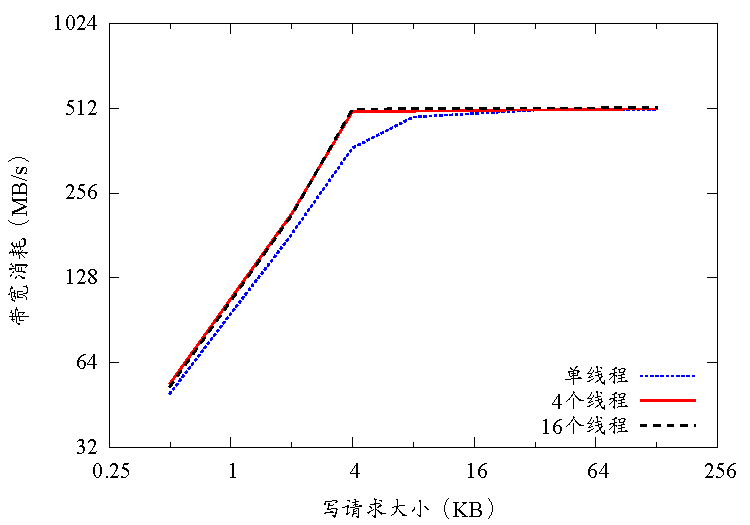
\includegraphics[width=0.9\columnwidth]{figures/nvme-bandwidth}
\caption{基于NVMe接口的Intel固态硬盘在不同写请求大小下的带宽消耗。}
\label{fig-nvme-bandwidth}
\end{figure}

图\ref{fig-nvme-bandwidth}绘制了一台PCIe NVMe接口的英特尔固态硬盘Intel SSD DC P3600在不同写请求大小下的带宽消耗。实验使用一台24核服务器,开启一定数量的线程直接像NVMe块设备连续发送固定大小的写请求。我们可以从曲线中得出两点观察。第一,峰值带宽达到500~MB/s,如果假设512~B的写入请求大小(YCSB负载的典型写大小),那么单台设备可支持每秒百万级的事务吞吐率。数据库在相同硬件配置下很难达到相同的吞吐率。第二,使用多个线程时,峰值带宽在写大小超过4~KB后即可达到,表明KB级别的缓冲区大小已经能够饱和利用存储设备性能,而该范围比为传统机械磁盘设计的缓冲区小两个数量级。小缓冲区可以在确认写完成时获得更小的延迟。

\section{系统实现}

\section{性能评测}

\section{本章小结}

总结起来,本章工作主要从三个方面推进了事务性内存接口下的持久性数据一致性机制。第一,我们提出了持久性事务性内存模型,为传统事务性内存增添了高效的持久性保证,将大容量的非易失性存储\emph{直接地}交由应用访问。第二,利用了我们事务性内存系统快照隔离的特性,将持久化的开销从只读负载的关键路径中移除。第三,考虑SSD和NVMe接口特性,设计了新的日志机制,小缓冲区组技术,同时达到高吞吐率和低延迟。


